\chapter{RESEARCH DESIGN}
\label{ch:research}

\section{Data Collection Methods}
\label{sec:datacollection}

\subsection{Candidate pairs and the frozen benchmark}

Candidate pairs are produced by the Curriculum Intelligence pipeline itself, as the pairs its rules leave open. Each candidate has a left side (the term found in a posting or curriculum, with its context lines), a right side (an ESCO concept with its description and hierarchy, or a curriculum topic), and metadata. Every context line carries an identifier (\code{L1}, \code{R1}, \ldots) and a source type such as \code{SOURCE\_TEXT}, \code{JOB\_TITLE}, \code{COURSE\_TITLE}, \code{UNIT\_TITLE}, \code{LEARNING\_OUTCOME}, \code{ESCO\_DESCRIPTION} or \code{ESCO\_HIERARCHY}. Taxonomy and normalisation facts are shown to the model only as metadata items and may never be cited as evidence. The frozen candidate file for the evaluated runs contains 283 candidates (SHA-256 \code{a889097d\ldots}).

The benchmark \code{semantic\_benchmark\_v1} selects 88 of these candidates and was frozen on 2026-09-27 (SHA-256 \code{94b4e79c\ldots}). Its cases belong to four kinds:
\begin{itemize}
    \item \code{ALIAS\_SENSE}: is a short or alternative form used in the sense of the ESCO concept?
    \item \code{AMBIGUOUS\_TAXONOMY\_LABEL}: which of several ESCO concepts sharing a label is meant?
    \item \code{AMBIGUOUS\_TOPIC\_MAPPING}: how does a curriculum topic relate to a candidate concept?
    \item \code{DIAGNOSTIC}: hard cases chosen to probe specific failure modes.
\end{itemize}
Each case also carries a development label, written by an AI assistant (Claude) under a documented protocol and marked \code{DEVELOPMENT\_GOLD\_ASSISTANT\_ADJUDICATED}. The freeze manifest records a known bias: the labeller had seen the outputs of an earlier model run for 75 of the cases before labelling. In this report, development labels are used only to stratify the human-validation subset and for development diagnostics. They are never a reference for accuracy.

\subsection{The 48-case human-validation subset}

Human validation uses 48 of the 88 cases. The selection (\code{semantic\_validation.py}, function \code{select\_subset}, seed \code{semantic-validation-v1}) is deterministic and uses no model output:
\begin{enumerate}
    \item quotas per case kind proportional to the benchmark (largest-remainder allocation);
    \item within a kind, cases spread proportionally over the development labels, keeping every label that occurs in the benchmark;
    \item failure-mode tags (lexical collision, acronym, hierarchy, abbreviation, alias, paraphrase) kept represented by swaps within the same cell;
    \item order inside a cell given by SHA-256 of the seed and the case identifier.
\end{enumerate}
Table~\ref{tab:benchmark} shows the resulting composition.

\begin{table}[H]
\centering
\begin{tabular}{@{}lrrr@{}}
\toprule
\textbf{Case kind} & \textbf{Benchmark (88)} & \textbf{Subset (48)} & \textbf{Scored (45)} \\
\midrule
\code{ALIAS\_SENSE} & 45 & 25 & 24 \\
\code{AMBIGUOUS\_TAXONOMY\_LABEL} & 18 & 10 & 8 \\
\code{AMBIGUOUS\_TOPIC\_MAPPING} & 12 & 6 & 6 \\
\code{DIAGNOSTIC} & 13 & 7 & 7 \\
\midrule
Total & 88 & 48 & 45 \\
\bottomrule
\end{tabular}
\caption[{Composition of the benchmark, the validation subset and the scored cases}]{Composition of the frozen benchmark, the human-validation subset, and the 45 cases scored against the R02/R03 agreement. Sources: \code{FREEZE\_MANIFEST.json}, \code{subset.json}, recomputed from the response files.}
\label{tab:benchmark}
\end{table}

\subsection{The reviewer form}

The subset was rendered as a Google Form, generated from the package files. Each case page shows Concept A with every context line of the benchmark case, verbatim and labelled by source, Concept B with its description and hierarchy (or curriculum lines), and three questions: the relationship (choices A--H, mapped to the eight labels of Table~\ref{tab:labels}), a confidence (High, Moderate, Low) and an optional reasoning. The form collects only a reviewer identifier. It never shows a development label, a case kind or tag, a model prediction, a confidence, the gate, or any indication of correctness. A generated integrity check confirms that every evidence line appears verbatim and that no label code, case kind or model name appears in the visible text.

\subsection{The reviewer response workbook}

One workbook of responses exists: \code{Semantic\_Relationship\_Validation\_R01\_to\_R05.xlsx}, SHA-256 \code{3d9eae28\ldots49ae04}. This hash was verified for this report on the attached copy. Its single sheet, \emph{Form responses 1}, has 146 columns (timestamp, reviewer identifier, and three columns for each of the 48 cases) and five data rows, R01 to R05. All 240 relationship answers parse to valid labels and all have a confidence, so the import recorded every answer as \code{COMPLETED}. All five rows carry the same timestamp, 2026-10-22 09:03:53.725. Separate form submissions would normally have distinct timestamps, which indicates that the rows were assembled into one sheet rather than exported submission by submission. The import records this.

The answering process was recorded at import as stated by the project owner on 2026-10-22 (Table~\ref{tab:reviewers}). R02 and R03 read about the topics with an AI assistant and then chose their answers; they are recorded as \code{HUMAN\_AI\_ASSISTED}. How R01, R04 and R05 answered was not stated (\code{NOT\_STATED}). Every record is stored with \code{counts\_as\_independent\_label = false}, with the raw cell text, the file hash, the sheet, row and cell, and the timestamp. The independent-label folder of the package (\code{labels/\allowbreak{}}) contains no file.

\begin{table}[H]
\centering
\begin{tabular}{@{}lllr@{}}
\toprule
\textbf{Reviewer} & \textbf{Recorded source} & \textbf{Independent label} & \textbf{Completed} \\
\midrule
R01 & \code{NOT\_STATED} & no & 48 / 48 \\
R02 & \code{HUMAN\_AI\_ASSISTED} & no & 48 / 48 \\
R03 & \code{HUMAN\_AI\_ASSISTED} & no & 48 / 48 \\
R04 & \code{NOT\_STATED} & no & 48 / 48 \\
R05 & \code{NOT\_STATED} & no & 48 / 48 \\
\bottomrule
\end{tabular}
\caption[{Reviewer records available}]{Reviewer records available. Source: \code{responses/responses\_r0\{1..5\}\_v1.json}.}
\label{tab:reviewers}
\end{table}

\subsection{Stored model predictions}

Two recorded model runs are evaluated. Both used \code{qwen2.5:7b-instruct} (7.6B parameters, Q4\_K\_M quantisation, model digest \code{845dbda0\ldots}) through Ollama 0.34.4 at temperature 0, with decision schema \code{decision-schema-v2}.
\begin{itemize}
    \item \textbf{v3} (\code{data/\allowbreak{}semantic\_runs/\allowbreak{}qwen-270-v3}): prompt \code{adjudicate-v3}, the production prompt; all 283 frozen candidates (which include the 88 benchmark cases). 283 model calls with no invalid output, 3001.1~s in total, median latency 10.5~s per decision. On a repeated subset of 20 candidates, all 20 returned the same relationship, and 17 the identical output.
    \item \textbf{v4} (\code{data/\allowbreak{}semantic\_runs/\allowbreak{}qwen-270-v4}): prompt \code{adjudicate-v4}, an experiment run on the 88 benchmark candidates only (2026-10-22). 88 model calls with no invalid output, 850.2~s, median latency 9.9~s. On the repeated subset, 20 of 20 returned the same relationship, and 16 the identical output.
\end{itemize}
Each decision record carries the provider, model, prompt version, input and context hashes, output hash, relationship, reason, cited evidence, alternatives and uncertainty, together with \code{is\_human\_validated = false}.

\section{Data Analysis Techniques}
\label{sec:analysis}

\subsection{Reference answers}

Because no independent label set exists, model answers are scored against a \emph{development reference}: the cases on which R02 and R03 gave the same label. This is the reference the project's scoring script (\code{scripts/\allowbreak{}semantic/\allowbreak{}score\_against\_reviewers.py}) builds, and it is labelled there as ``not independent labels''. R02 and R03 are the script's default pair and the only two reviewers whose answering process was stated. That stated process (AI-assisted) is why the reference is development-only.

\subsection{Raw, validated and committed answers}

For each case the model's \emph{raw} answer is the relationship it returned. The \emph{validated} answer is what downstream could read after the evidence validator (Section~\ref{sec:impl}): the relationship if the validator returns \code{MODEL\_SUPPORTED} or \code{MODEL\_SUGGESTED}; \IE{} if the relationship lacks required evidence; and \AM{} if the evidence cannot be traced to the inputs or the decision failed. A validated answer is a \emph{commitment} when it is one of the six definite labels (\SC, \PA, \CH, \RE, \PO, \UN). A validated \AM{} or \IE{} is an \emph{abstention}.

\subsection{Metrics}

Let $N$ be the number of scored cases, $y_i$ the reference label and $\hat{y}_i$ the system's label for case $i$, and $C$ the set of cases on which the system commits.

\begin{align}
\text{Exact-match accuracy} &= \frac{1}{N}\sum_{i=1}^{N} \mathbb{1}[\hat{y}_i = y_i] \label{eq:acc}\\
\text{Coverage} &= \frac{|C|}{N}, \qquad \text{Abstention rate} = 1 - \text{Coverage} \label{eq:cov}\\
\text{Conditional accuracy} &= \frac{1}{|C|}\sum_{i \in C} \mathbb{1}[\hat{y}_i = y_i] \label{eq:condacc}
\end{align}

Exact-match accuracy counts an abstention as wrong unless the reference itself is \AM{} or \IE. On this reference no abstention matched, so every correct validated answer is a commitment. Conditional accuracy is the accuracy on the cases where the system commits, the quantity a downstream user relies on. For each class $c$, precision $P_c$, recall $R_c$ and $F1_c = 2P_cR_c/(P_c+R_c)$ are computed from the confusion matrix. Precision is undefined when the class is never predicted. Macro-F1 is the mean over the classes present in the reference, counting an undefined F1 as 0.

Agreement between two reviewers $a$ and $b$ over $n$ cases is reported as raw agreement $p_o$ and Cohen's $\kappa$~\cite{cohen1960}:
\begin{equation}
\kappa = \frac{p_o - p_e}{1 - p_e}, \qquad p_e = \sum_{c} \frac{n_{a,c}\, n_{b,c}}{n^2},
\label{eq:kappa}
\end{equation}
where $n_{a,c}$ is the number of cases reviewer $a$ labelled $c$. Proportions are given with 95\% Wilson score intervals~\cite{wilson1927} to show how little a sample of 45 can establish:
\begin{equation}
\frac{\hat{p} + \frac{z^2}{2n}}{1+\frac{z^2}{n}} \pm \frac{z}{1+\frac{z^2}{n}}\sqrt{\frac{\hat{p}(1-\hat{p})}{n} + \frac{z^2}{4n^2}}, \qquad z = 1.96.
\label{eq:wilson}
\end{equation}

\subsection{Error categories and the baseline}

An error is a case where the raw answer differs from the reference. It is named by the pair (reference $\rightarrow$ answer), for example \CH~$\rightarrow$~\SC. Each case has one reference and one raw answer, so these categories are disjoint and their counts can be summed. The \emph{fixed-rule baseline} is the deterministic system's verdict on the same candidates. By construction it is \AM{} for every candidate it handles, since candidates exist only because the rules could not decide. It is not produced for \code{DIAGNOSTIC} cases.

\subsection{The promotion gates}

Two gates govern the model, and both were declared before the outputs they judge were known.

\paragraph{Development gate (v3 run).} Declared in \code{engine\_config.json} on 2026-09-27, before any v3 output existed. It is applied to the 88-case benchmark with its development labels, and it governs whether model decisions on \code{ALIAS\_SENSE} candidates may establish (\SC) or reject (\UN) an alias mention. The v3 run failed it (Section~\ref{sec:results}).

\paragraph{Human-validation gate (semantic-gate-v3).} Declared on 2026-09-29, when no independent label file existed, and pinned by SHA-256 (\code{399b4cfa\ldots}) in \code{engine\_config.json}. It evaluates the validated system on the frozen gold set built from independent labels. Table~\ref{tab:gate} lists its criteria. If any criterion fails, the system stays in Safe Mode. If all pass, only those classes among \SC, \UN, \PA, \CH, \RE{} with at least 8 predictions and precision of at least 0.90 may take effect. Any change to the gate must be declared as a new version before the results it is applied to are seen.

\begin{table}[H]
\centering
\small
\begin{tabular}{@{}lr@{}}
\toprule
\textbf{Criterion} & \textbf{Threshold} \\
\midrule
Independent human reviewers & $\geq 2$ \\
Gold cases (unanimous or adjudicated) & $\geq 44$ \\
Cohen's $\kappa$ between reviewers & $\geq 0.60$ \\
Accuracy of the validated system & $\geq 0.80$ \\
Macro-F1 of the validated system & $\geq 0.70$ \\
False \SC{} & $\leq 1$ \\
Wrong hierarchy direction & $0$ \\
False \PA{} or \CH{} & $\leq 1$ \\
Unsupported taxonomy evidence & $0$ \\
Lexical collisions & $0$ \\
Predictions per promoted class & $\geq 8$ \\
Precision per promoted class & $\geq 0.90$ \\
\bottomrule
\end{tabular}
\caption[{Criteria of semantic-gate-v3}]{Criteria of semantic-gate-v3 (\code{data/\allowbreak{}evaluation/\allowbreak{}semantic\_gate\_v3.json}).}
\label{tab:gate}
\end{table}

\section{Project Design and Development}
\label{sec:projectdesign}

\subsection{Place of the module in the Curriculum Intelligence pipeline}

The pipeline is organised in layers: hash-verified sources; a bronze layer of page text; a silver layer of courses, units, topics and postings with data contracts and quarantine; a health gate; and a gold layer of concepts, mappings, ESCO-linked skills, demand, gaps and recommendations. It is published to PostgreSQL and served read-only through a FastAPI back end to a Flutter front end. Semantic adjudication sits inside the gold layer's intelligence stage. Figure~\ref{fig:architecture} shows the flow of a candidate through the module.

\begin{figure}[H]
\centering
\resizebox{\textwidth}{!}{%
\begin{tikzpicture}[
  node distance=0.55cm and 0.6cm,
  box/.style={draw, rounded corners=2pt, align=center, font=\footnotesize, minimum height=0.95cm, text width=3.3cm, fill=white},
  rule/.style={box, fill=gray!12},
  model/.style={box, fill=blue!8},
  gate/.style={box, fill=orange!12},
  arr/.style={-{latex}, thick}]
\node[box] (rules) {Deterministic rules\\(ESCO labels, alias/acronym sense, containment)};
\node[box, right=of rules] (cand) {Open candidate pairs\\(context items with ids and source types)};
\node[model, right=of cand] (prov) {Model provider\\Qwen2.5 7B via Ollama\\prompt \code{adjudicate-v3}};
\node[box, below=of prov] (dec) {Decision record\\(label, reason, evidence, hashes)};
\node[rule, left=of dec] (val) {Evidence validator\\(\code{validate\_decision})};
\node[gate, left=of val] (gate) {Promotion gate\\(declared in advance)};
\node[box, below=0.9cm of gate, text width=3.6cm] (safe) {\textbf{Safe Mode} (current)\\recorded and shown,\\never applied};
\node[box, below=0.9cm of val, text width=3.6cm] (eff) {Effect on analysis\\(only promoted classes,\\only if the gate passes)};
\node[box, below=0.9cm of dec] (cache) {Replay cache\\(exact key: prompt, schema,\\model, input/context hash)};
\draw[arr] (rules) -- node[above, font=\scriptsize]{undecided} (cand);
\draw[arr] (cand) -- (prov);
\draw[arr] (prov) -- (dec);
\draw[arr] (dec) -- (val);
\draw[arr] (val) -- (gate);
\draw[arr] (gate) -- node[left, font=\scriptsize]{fails} (safe);
\draw[arr, dashed] (gate.south east) -- node[right, font=\scriptsize, pos=0.4]{passes} (eff.north west);
\draw[arr] (dec) -- (cache);
\end{tikzpicture}}
\caption[{Flow of a candidate pair through the semantic adjudication module}]{Flow of a candidate pair through the semantic adjudication module (from \code{docs/\allowbreak{}SEMANTIC\_INTELLIGENCE.md}, \code{semantic\_provider.py}, \code{semantic\_v3.py} and \code{engine\_config.json}). The dashed path has never been taken.}
\label{fig:architecture}
\end{figure}

\subsection{The validation workflow}

Figure~\ref{fig:workflow} shows the validation workflow. Its left branch, from the frozen benchmark through the blinded form, was carried out up to the reviewer responses. Its right branch, from independent labels through agreement, adjudication, frozen gold and gate evaluation, is implemented in \code{scripts/\allowbreak{}evaluation/\allowbreak{}semantic\_validation.py} but has not run, because no independent label set exists. The development scoring of this report is the middle path.

\begin{figure}[H]
\centering
\resizebox{\textwidth}{!}{%
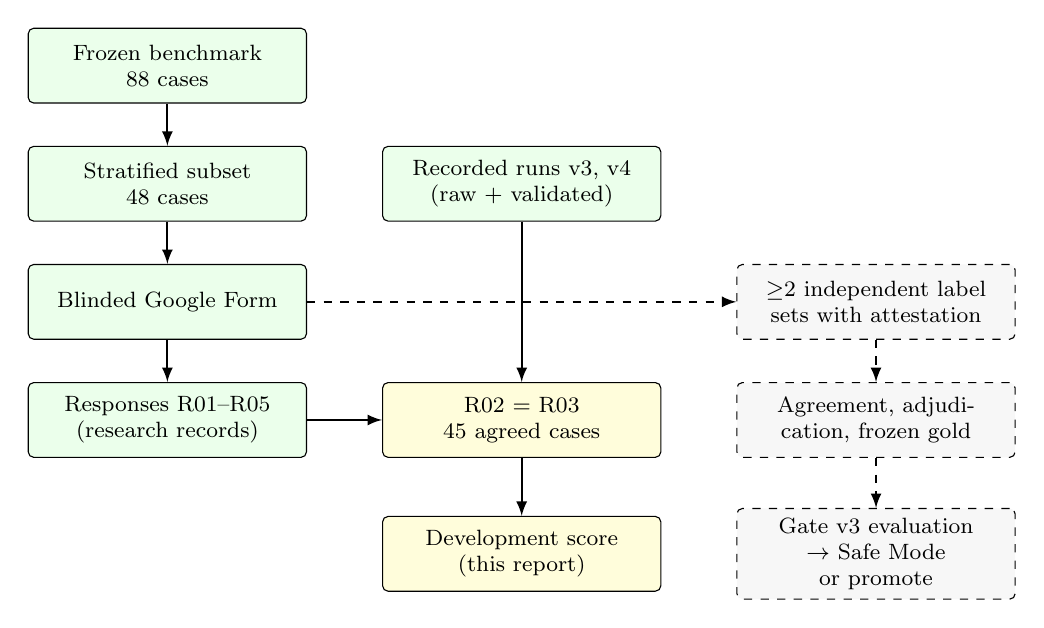
\begin{tikzpicture}[
  box/.style={draw, rounded corners=2pt, align=center, font=\footnotesize, minimum height=0.95cm, text width=3.3cm},
  done/.style={box, fill=green!8},
  dev/.style={box, fill=yellow!14},
  todo/.style={box, dashed, fill=gray!6},
  arr/.style={-{latex}, thick}]
% column 1: carried out
\node[done] (bench) at (0,0) {Frozen benchmark\\88 cases};
\node[done] (sub)   at (0,-1.5) {Stratified subset\\48 cases};
\node[done] (form)  at (0,-3.0) {Blinded Google Form};
\node[done] (resp)  at (0,-4.5) {Responses R01--R05\\(research records)};
% column 2: development scoring (this report)
\node[done] (runs)  at (4.5,-1.5) {Recorded runs v3, v4\\(raw + validated)};
\node[dev]  (agree) at (4.5,-4.5) {R02 = R03\\45 agreed cases};
\node[dev]  (score) at (4.5,-6.2) {Development score\\(this report)};
% column 3: not yet run
\node[todo] (ind)   at (9,-3.0) {$\geq$2 independent label sets with attestation};
\node[todo] (gold)  at (9,-4.5) {Agreement, adjudication, frozen gold};
\node[todo] (eval)  at (9,-6.2) {Gate v3 evaluation\\$\rightarrow$ Safe Mode or promote};
\draw[arr] (bench) -- (sub);
\draw[arr] (sub) -- (form);
\draw[arr] (form) -- (resp);
\draw[arr] (resp) -- (agree);
\draw[arr] (agree) -- (score);
\draw[arr] (runs) -- (agree);
\draw[arr, dashed] (form) -- (ind);
\draw[arr, dashed] (ind) -- (gold);
\draw[arr, dashed] (gold) -- (eval);
\end{tikzpicture}}
\caption[{The validation workflow}]{The validation workflow. Solid boxes: carried out. Shaded boxes: the development scoring reported here. Dashed boxes: implemented but not yet run (no independent labels); the gate evaluation will score the same recorded runs.}
\label{fig:workflow}
\end{figure}

\subsection{Integration with the rest of the project}

Model decisions never become source evidence. In Safe Mode they are stored next to the rule verdict and shown in the application's \emph{Semantic decisions} screens, but they change no demand, coverage, gap or recommendation. When the pipeline host cannot reach the model, recorded decisions are replayed only by an exact cache key: prompt version, schema, model, input hash and context hash. The replayed run's own gate result still applies. Reviewer responses are reachable through \code{/\allowbreak{}api/\allowbreak{}v1/\allowbreak{}semantic-validation/\allowbreak{}} endpoints and a \emph{Reviewer validation} screen. A development label is shown there only as a field marked \code{is\_human\_judgment: false} and never enters a metric.
